\documentclass[10pt]{beamer}

\usetheme{default} % theme général du diaporama

% paquets pour le français
\usepackage[T1]{fontenc}
\usepackage[utf8]{inputenc}
\usepackage{graphicx}

% use serif font with rm
% \renewcommand{\familydefault}{\rmdefault}

\title{Spatially continuous identification of beta diversity hotspots using species distribution models}
\author{Gabriel Dansereau}

\begin{document}

\begin{frame}
  \titlepage
\end{frame}

\begin{frame}
  \frametitle{Objective}
  \begin{figure}
    \centering
    \hspace*{0.0cm}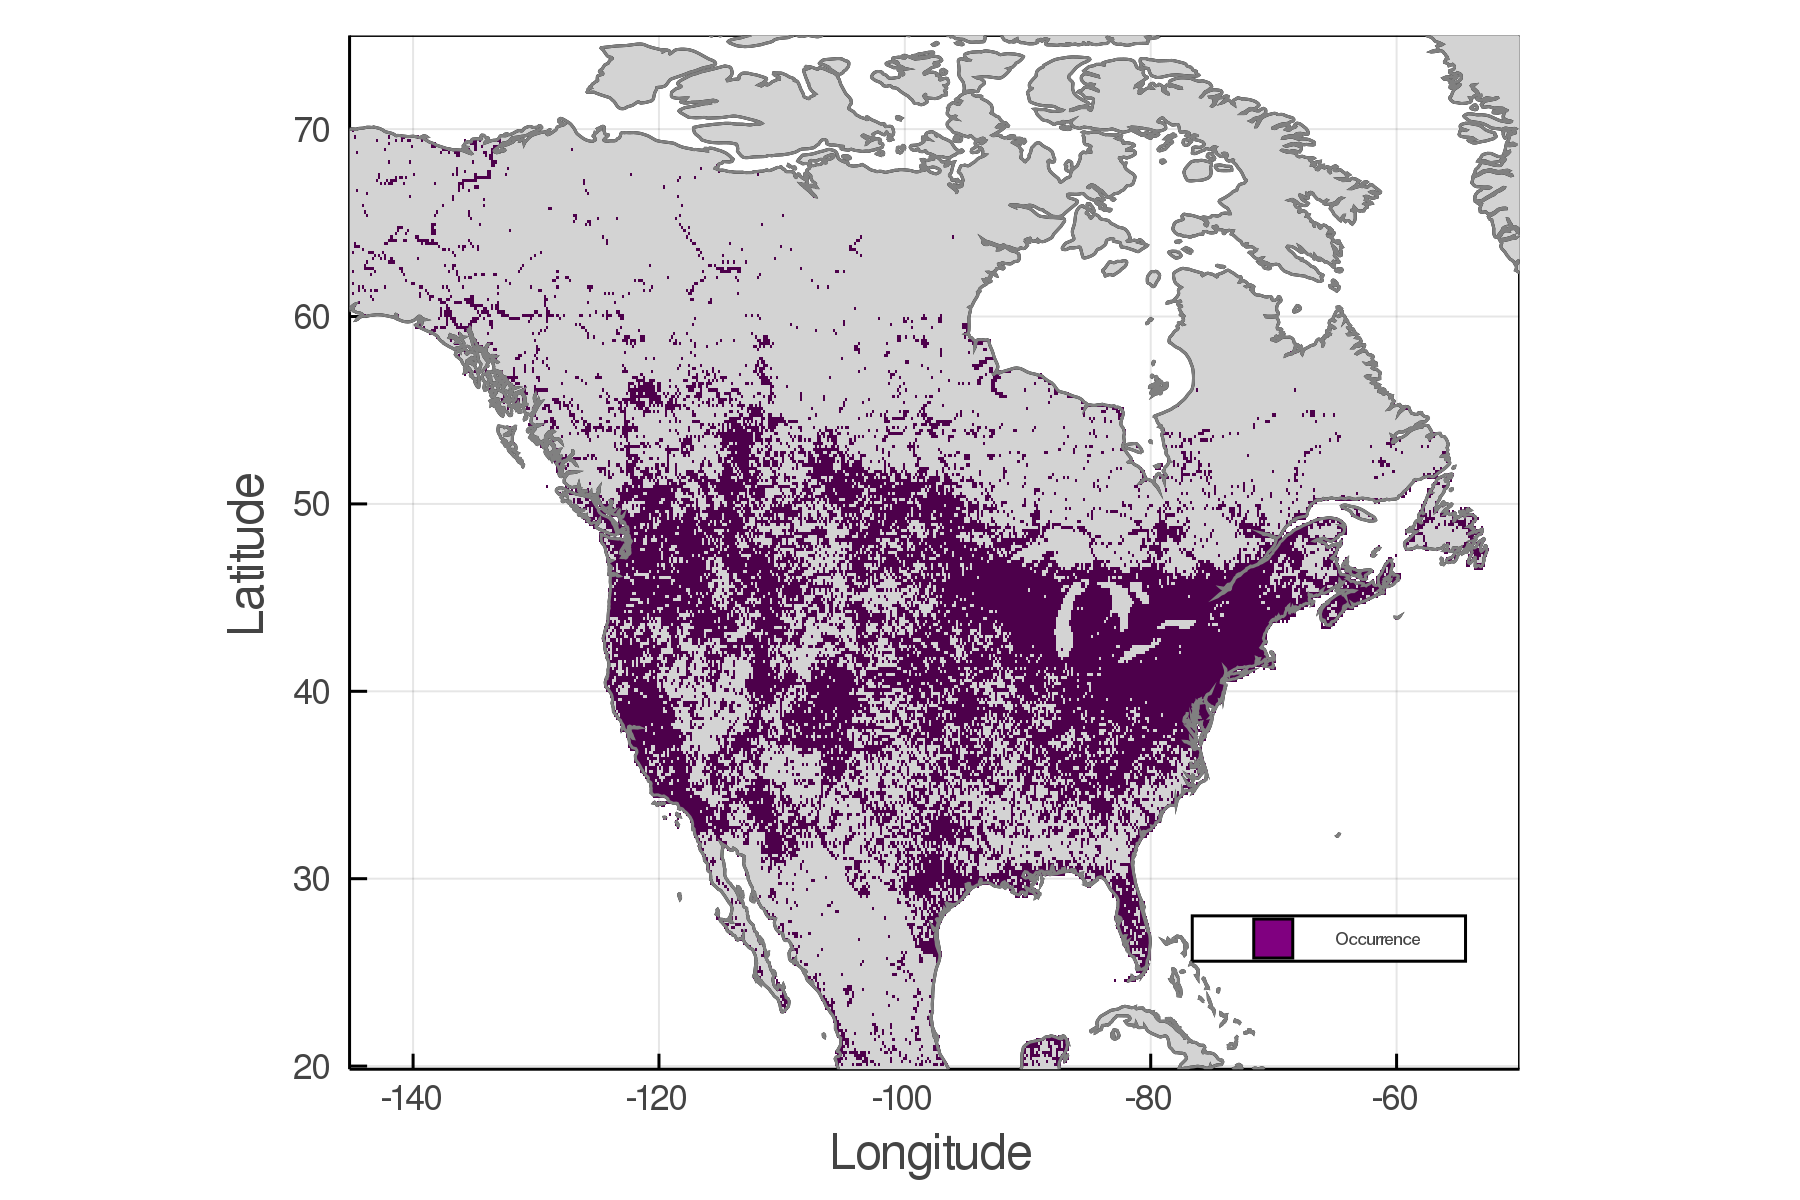
\includegraphics[scale=0.08]{fig/01_raw_singlesp.png}
    \hspace*{0.0cm}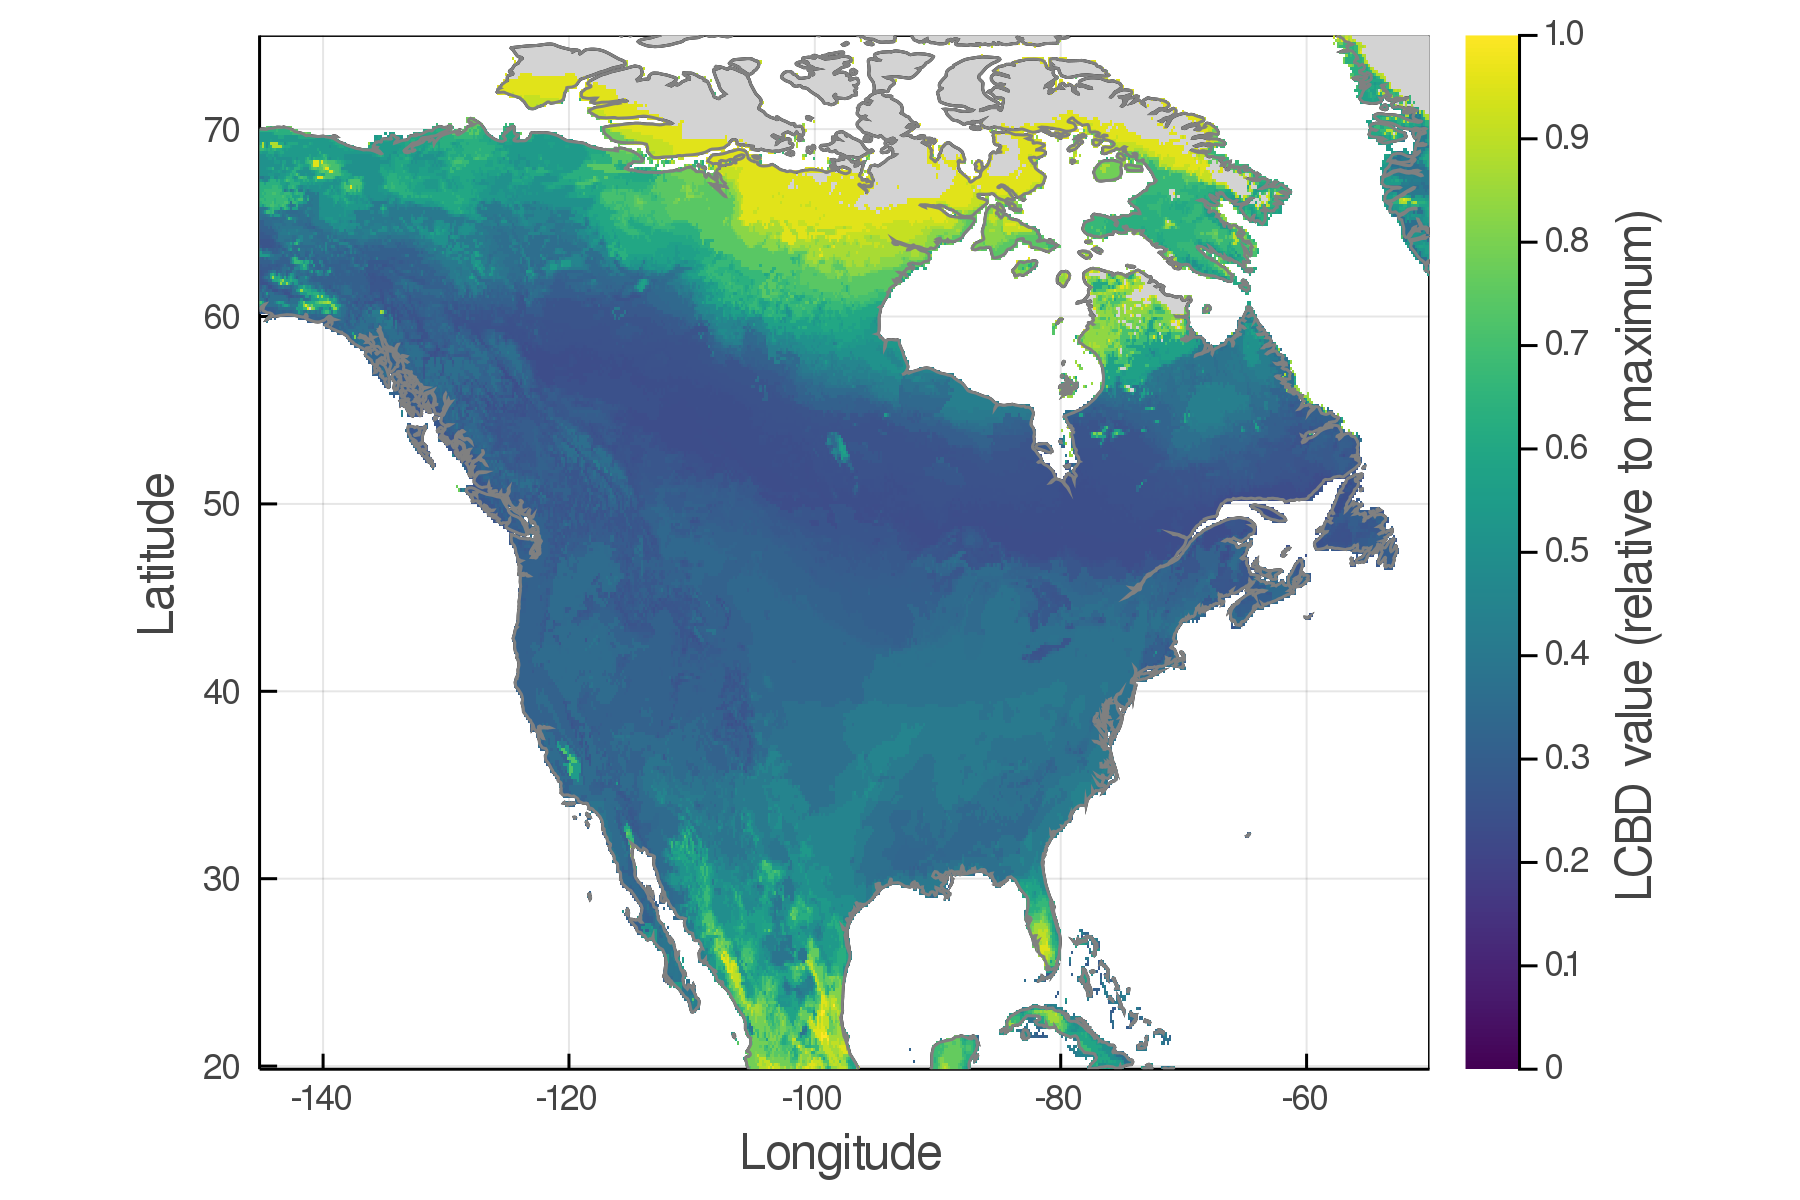
\includegraphics[scale=0.08]{fig/05_sdm_lcbd.png}
    \hspace{4.0cm}\begin{itemize}
      \item Beta diversity hotspots (LCBD)
      \item Species distribution models (SDM)
      \item Spatially continuous identification
    \end{itemize}
  \end{figure}
\end{frame}

\begin{frame}
  \frametitle{Ex 1. Discontinuous Identification of Beta Diversity Hotspots}
  \begin{figure}
    \centering
    \hspace*{-0cm}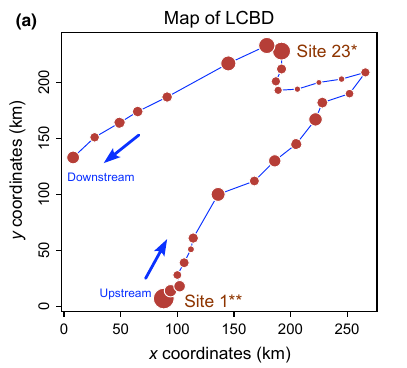
\includegraphics[scale=0.5]{fig/lcbd_LegeDeCa2013.png}
    \caption{Example of LCBD calculation on a river stream (Legendre \& De Caceres, 2013)}
  \end{figure}
\end{frame}

\begin{frame}
  \frametitle{Ex 2: Discontinuous Identification of Beta Diversity Hotspots}
  \begin{figure}
    \centering
    \hspace*{-0cm}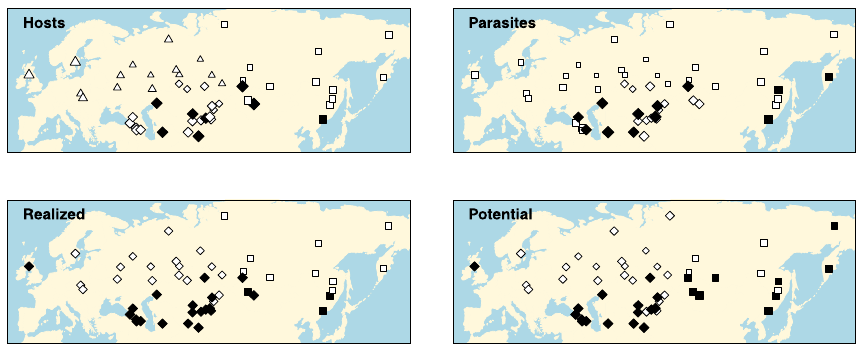
\includegraphics[scale=0.35]{fig/lcbd_Pois2017.png}
    \caption{Example of LCBD calculation on an extended scale (Poisot et al., 2017)}
  \end{figure}
\end{frame}

\begin{frame}
  \frametitle{Available Data}
  \begin{figure}
    \centering
    \hspace*{-0.5cm}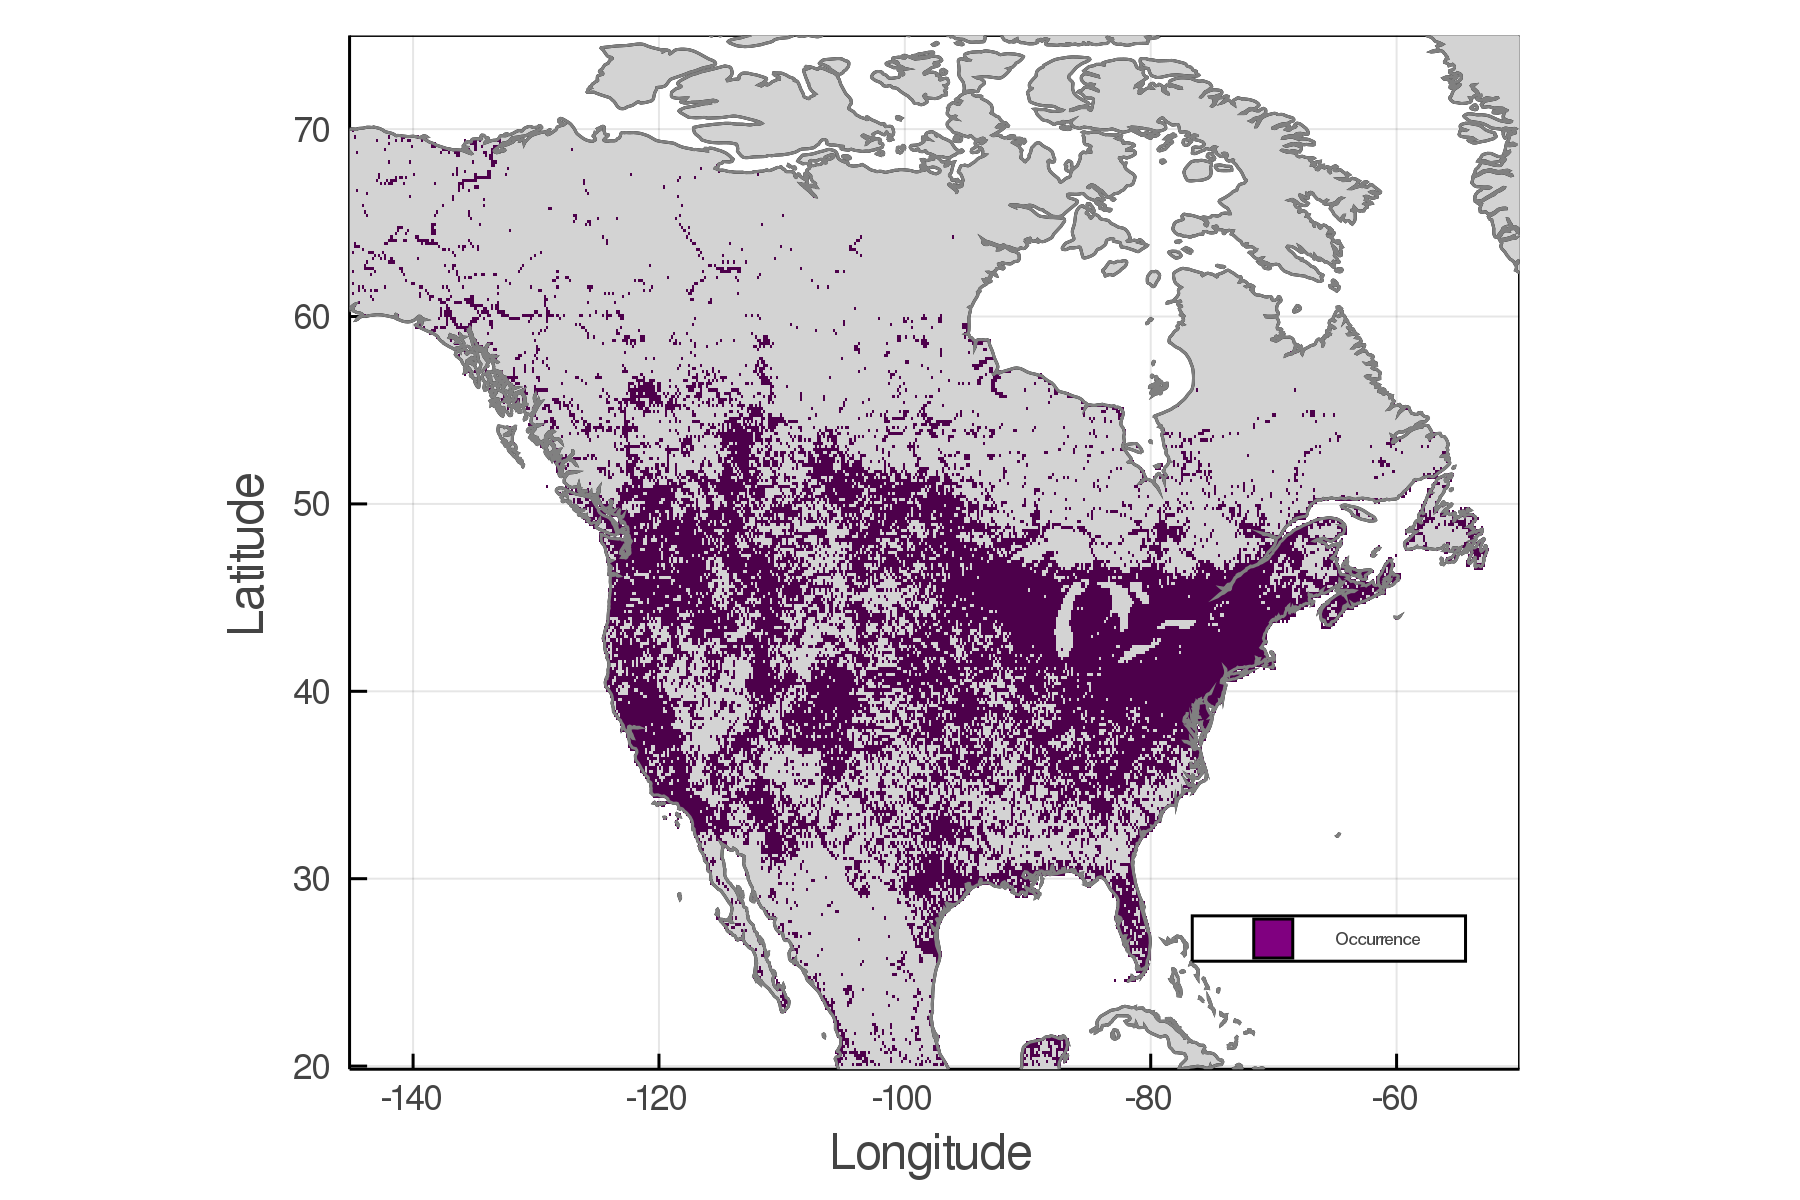
\includegraphics[scale=0.08]{fig/01_raw_singlesp.png}
    \hspace*{0.5cm}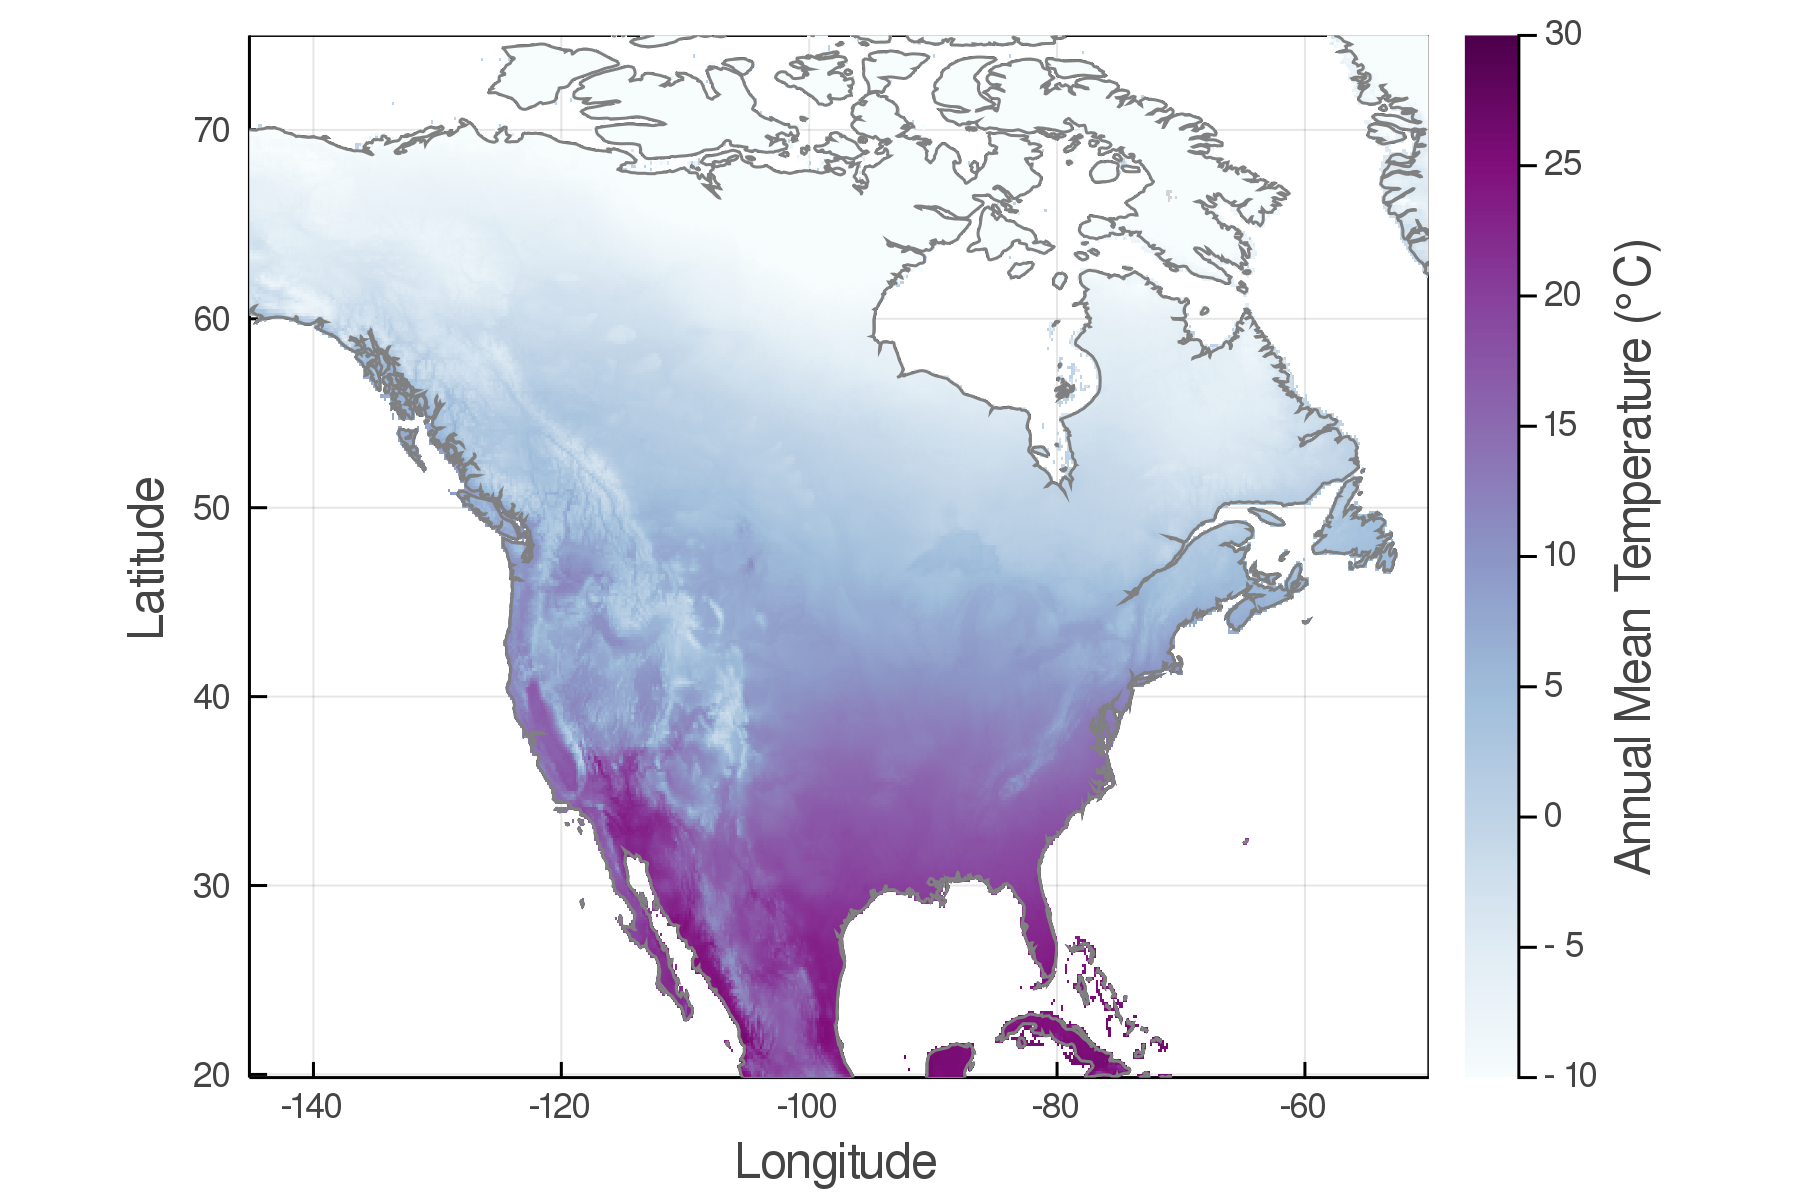
\includegraphics[scale=0.08]{fig/wc_temp.png}
  \end{figure}
\end{frame}

\begin{frame}
  \frametitle{Objective}
  \begin{figure}
    \centering
    \hspace*{-0cm}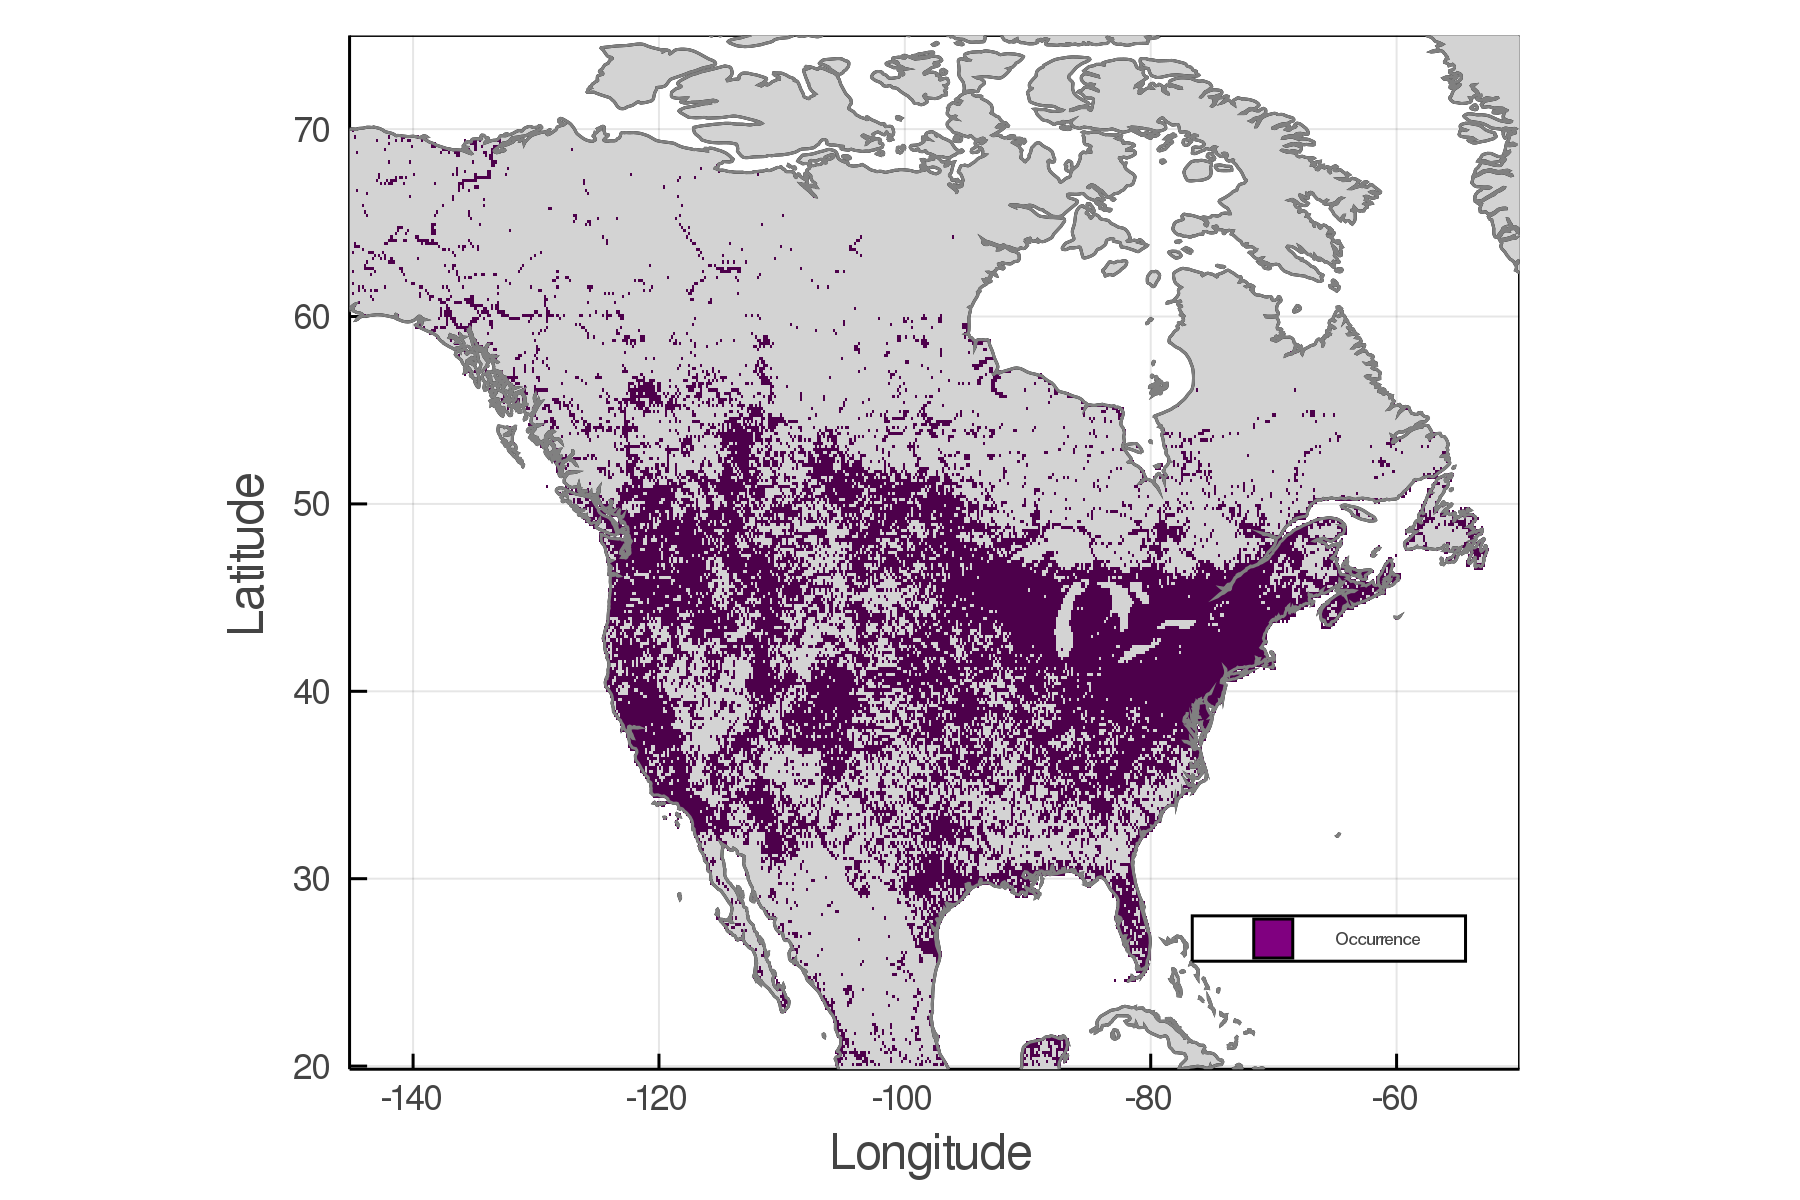
\includegraphics[scale=0.05]{fig/01_raw_singlesp.png}
    \hspace*{0cm}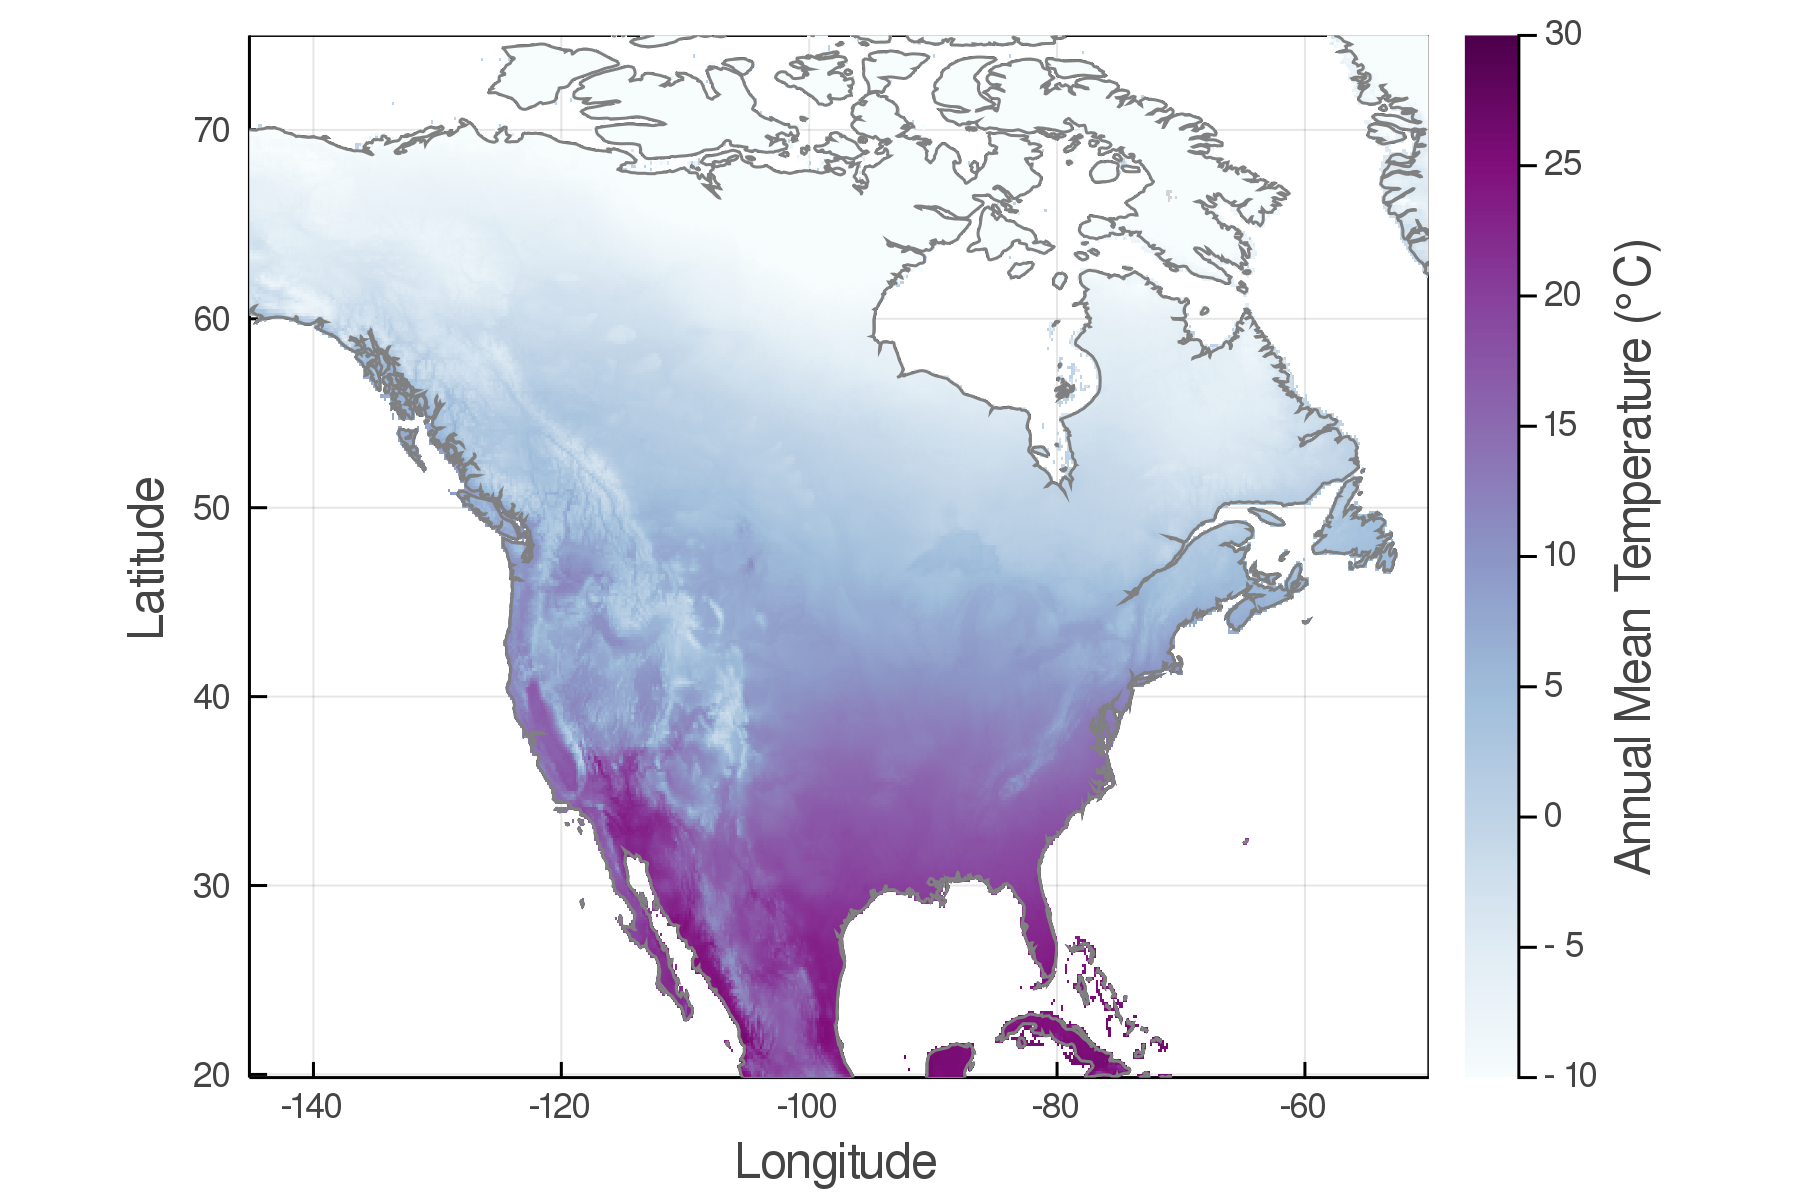
\includegraphics[scale=0.05]{fig/wc_temp.png}
    \vfill
    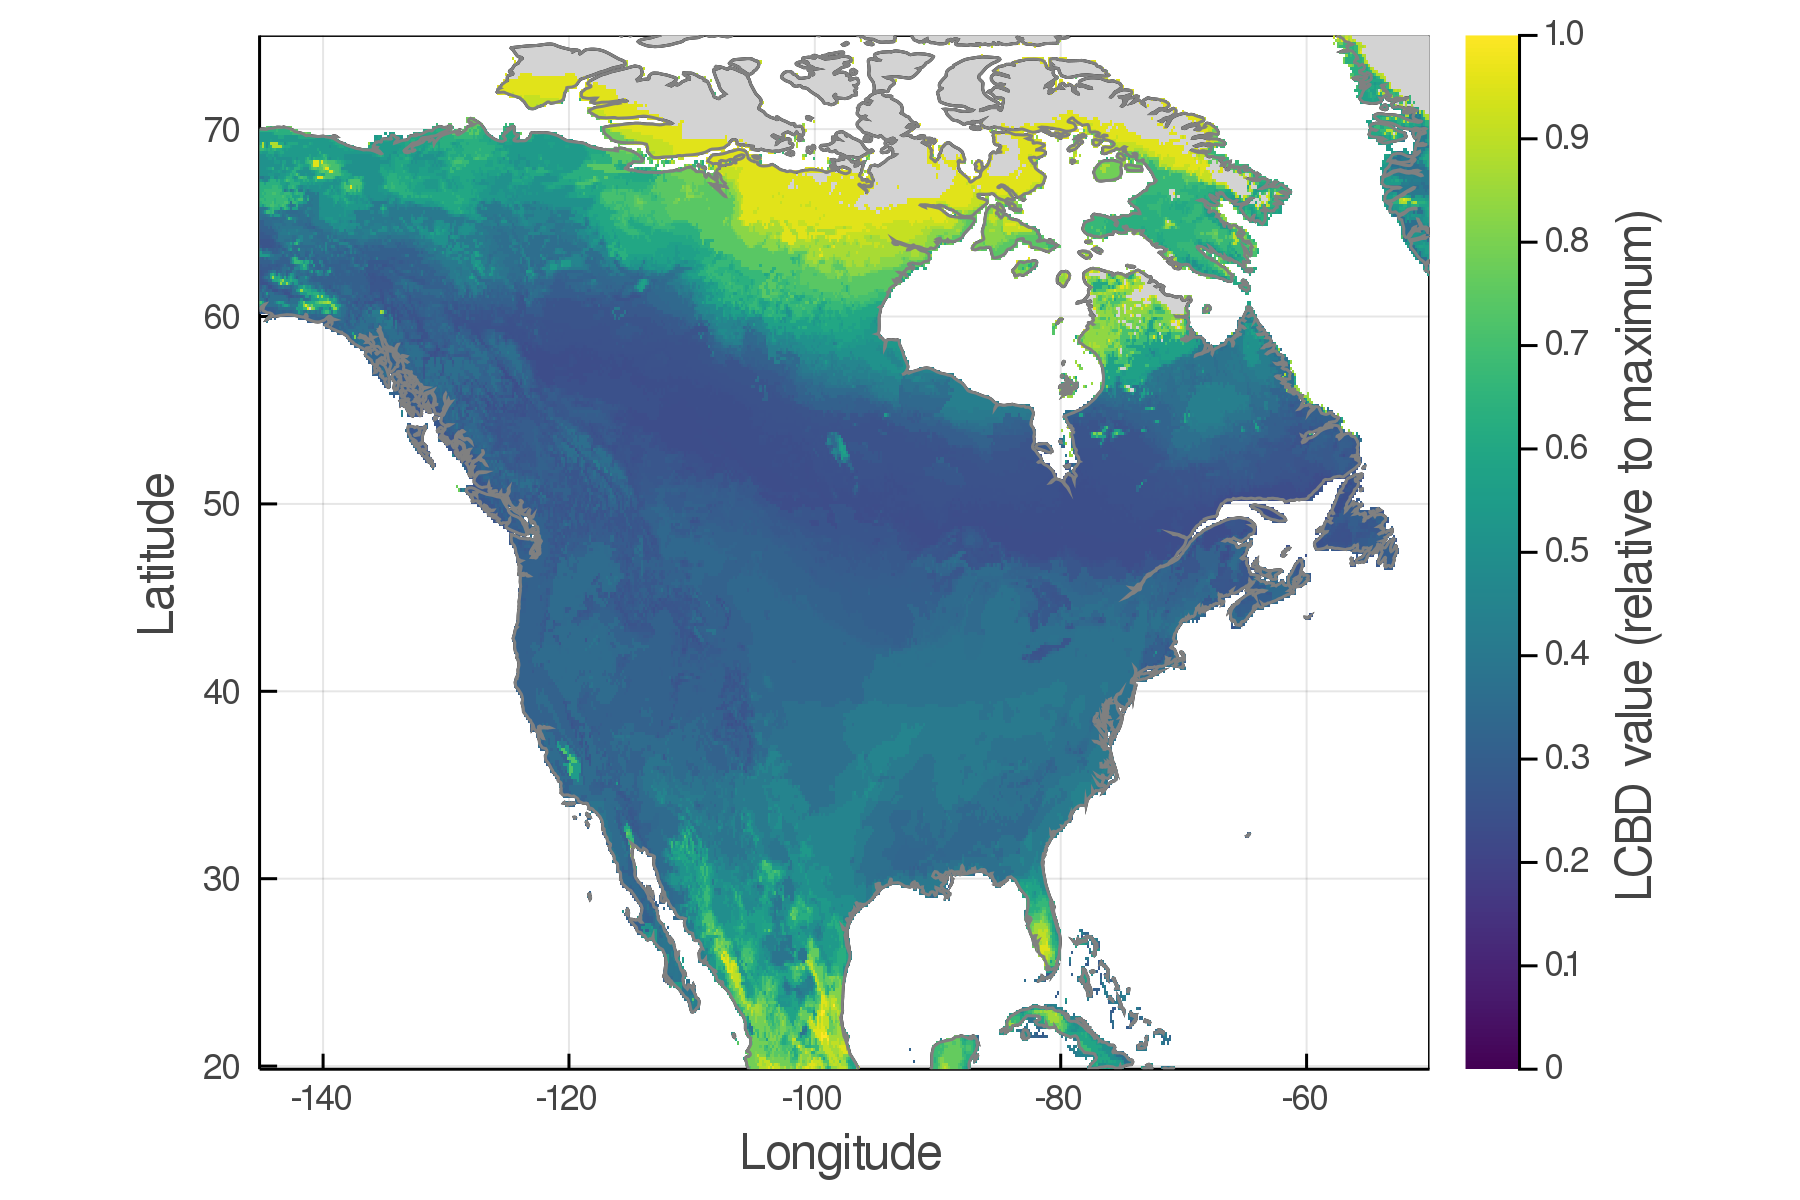
\includegraphics[scale=0.10]{fig/05_sdm_lcbd.png}
  \end{figure}
\end{frame}

\begin{frame}
  \frametitle{Data - eBird}
  \begin{itemize}
    \item Basis variables : species, latitude, longitude, date, complete checklist, abundance
  \end{itemize}
  \resizebox{\textwidth}{!}{%
  \begin{table}[ht]
    \centering
    \begin{tabular}{rlrrlrl}
      \small
      \hline
      obs & species & latitude & longitude & observationDate & allSpeciesReported &   observationCount \\
      \hline
      1 & Setophaga\_townsendi & 35.32 & -120.84 & 2007-03-17 &   1 & 1 \\
      2 & Geothlypis\_trichas & 35.32 & -120.84 & 1994-11-06 &   1 & 4 \\
      3 & Oreothlypis\_celata & 58.35 & -134.59 & 2008-07-22 &   1 & 2 \\
      4 & Setophaga\_coronata & 58.35 & -134.59 & 2008-07-22 &   1 & 1 \\
      5 & Setophaga\_coronata & 49.10 & -123.17 & 1979-10-16 &   1 & 8 \\
      6 & Setophaga\_coronata & 37.90 & -75.37 & 2004-11-23 &   1 & 82 \\
      \hline
    \end{tabular}
  \end{table}
  }
  \begin{itemize}
    \item Sampling: sampling type, duration, distance travelled, number of observers
  \end{itemize}
  \resizebox{\textwidth}{!}{%
    \begin{table}[ht]
      \centering
      \begin{tabular}{rlrrr}
        \small
        \hline
        & protocolType & durationMinutes & effortDistanceKm & numberObservers \\
        \hline
        1 & Area &  60 &  &  15 \\
        2 & Historical &  30 &  &   1 \\
        3 & Traveling &  50 & 2.09 &   1 \\
        4 & Traveling &  50 & 2.09 &   1 \\
        5 & Incidental &  &  &   1 \\
        6 & Traveling & 105 & 2.58 &   5 \\
        \hline
      \end{tabular}
    \end{table}
  }
\end{frame}

\begin{frame}
  \frametitle{Data - eBird}
  \begin{figure}
    \centering
    \hspace*{-0cm}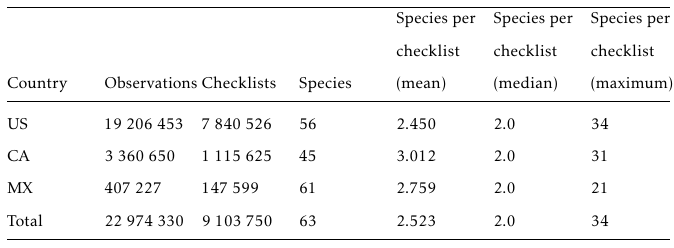
\includegraphics[scale=0.4]{fig/ebird_table.png}
  \end{figure}
\end{frame}

\begin{frame}
  \frametitle{Data - WorldClim}
  \resizebox{\textwidth}{!}{%
    \begin{table}
      \begin{tabular}{l|l}
        \small
        \hline
        Variable & Description                                                \\
        \hline
        1        & Annual Mean Temperature                                    \\
        2        & Mean Diurnal Range (Mean of monthly (max temp - min temp)) \\
        3        & Isothermality (BIO2/BIO7) (* 100)                          \\
        4        & Temperature Seasonality (standard deviation *100)          \\
        5        & Max Temperature of Warmest Month                           \\
        6        & Min Temperature of Coldest Month                           \\
        7        & Temperature Annual Range (BIO5-BIO6)                       \\
        8        & Mean Temperature of Wettest Quarter                        \\
        9        & Mean Temperature of Driest Quarter                         \\
        10       & Mean Temperature of Warmest Quarter                        \\
        11       & Mean Temperature of Coldest Quarter                        \\
        12       & Annual Precipitation                                       \\
        13       & Precipitation of Wettest Month                             \\
        14       & Precipitation of Driest Month                              \\
        15       & Precipitation Seasonality (Coefficient of Variation)       \\
        16       & Precipitation of Wettest Quarter                           \\
        17       & Precipitation of Driest Quarter                            \\
        18       & Precipitation of Warmest Quarter                           \\
        19       & Precipitation of Coldest Quarter                           \\
        \hline
      \end{tabular}
    \end{table}
  }
\end{frame}

\begin{frame}
  \frametitle{BIOCLIM}
  \begin{figure}
    \centering
    \hspace*{-0cm}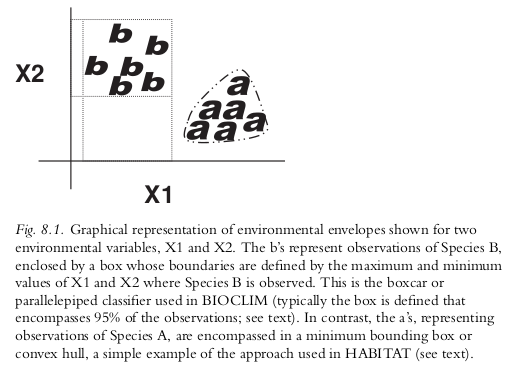
\includegraphics[scale=0.5]{fig/bioclim-with-caption.png}
  \end{figure}
\end{frame}

\begin{frame}
  \frametitle{Ex. Yellow Warbler - Raw Data}
  \begin{figure}
    \centering
    \hspace*{-0cm}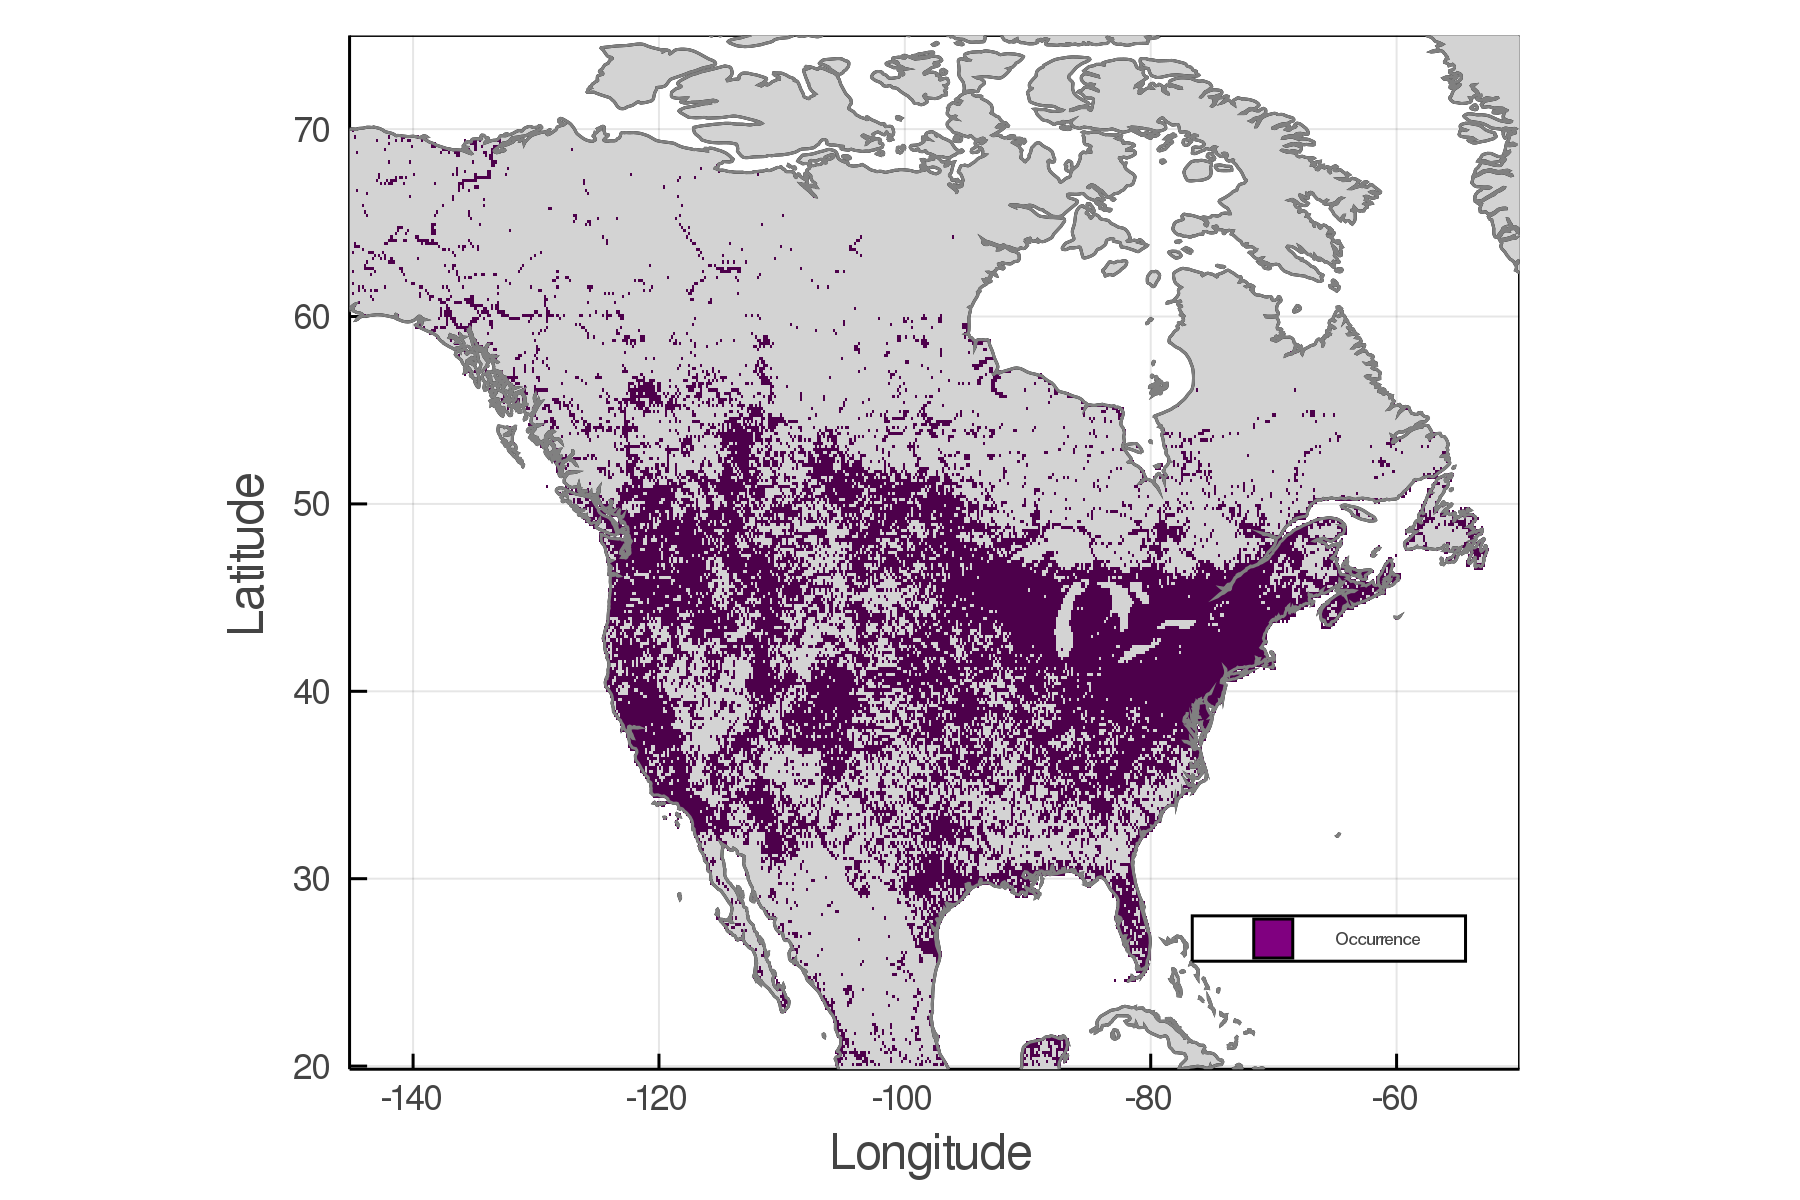
\includegraphics[scale=0.17]{fig/01_raw_singlesp.png}
    \caption{Yellow Warbler Distibution (presence-absence per site)}
  \end{figure}
\end{frame}

\begin{frame}
  \frametitle{Ex: Yellow Warbler - SDM with threshold}
  \begin{figure}
    \centering
    \hspace*{-0cm}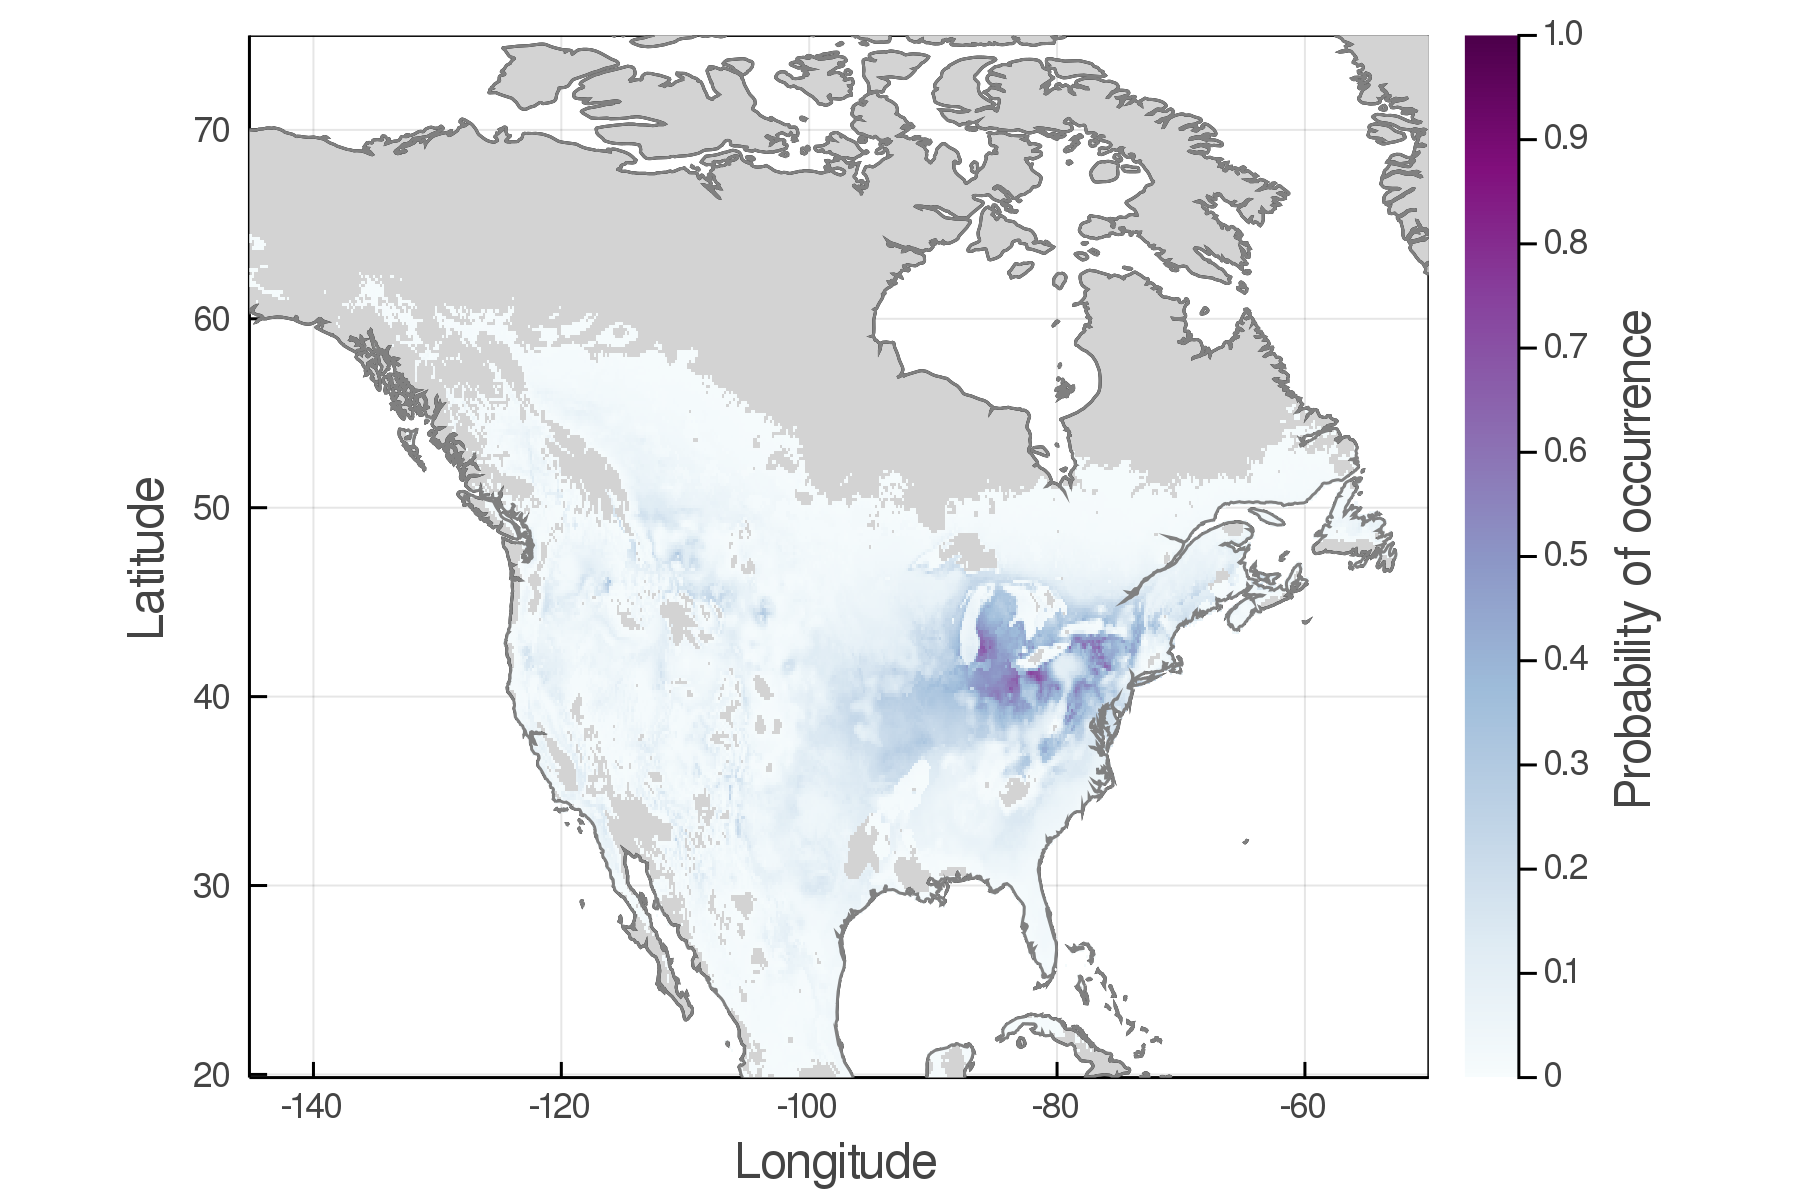
\includegraphics[scale=0.17]{fig/01_sdm_singlesp-threshold.png}
    \caption{SDM predictions with threshold (5\%) for the distribution of Yellow Warblers}
  \end{figure}
\end{frame}

\begin{frame}
  \frametitle{Ex: Yellow Warbler - SDM without threshold}
  \begin{figure}
    \centering
    \hspace*{-0cm}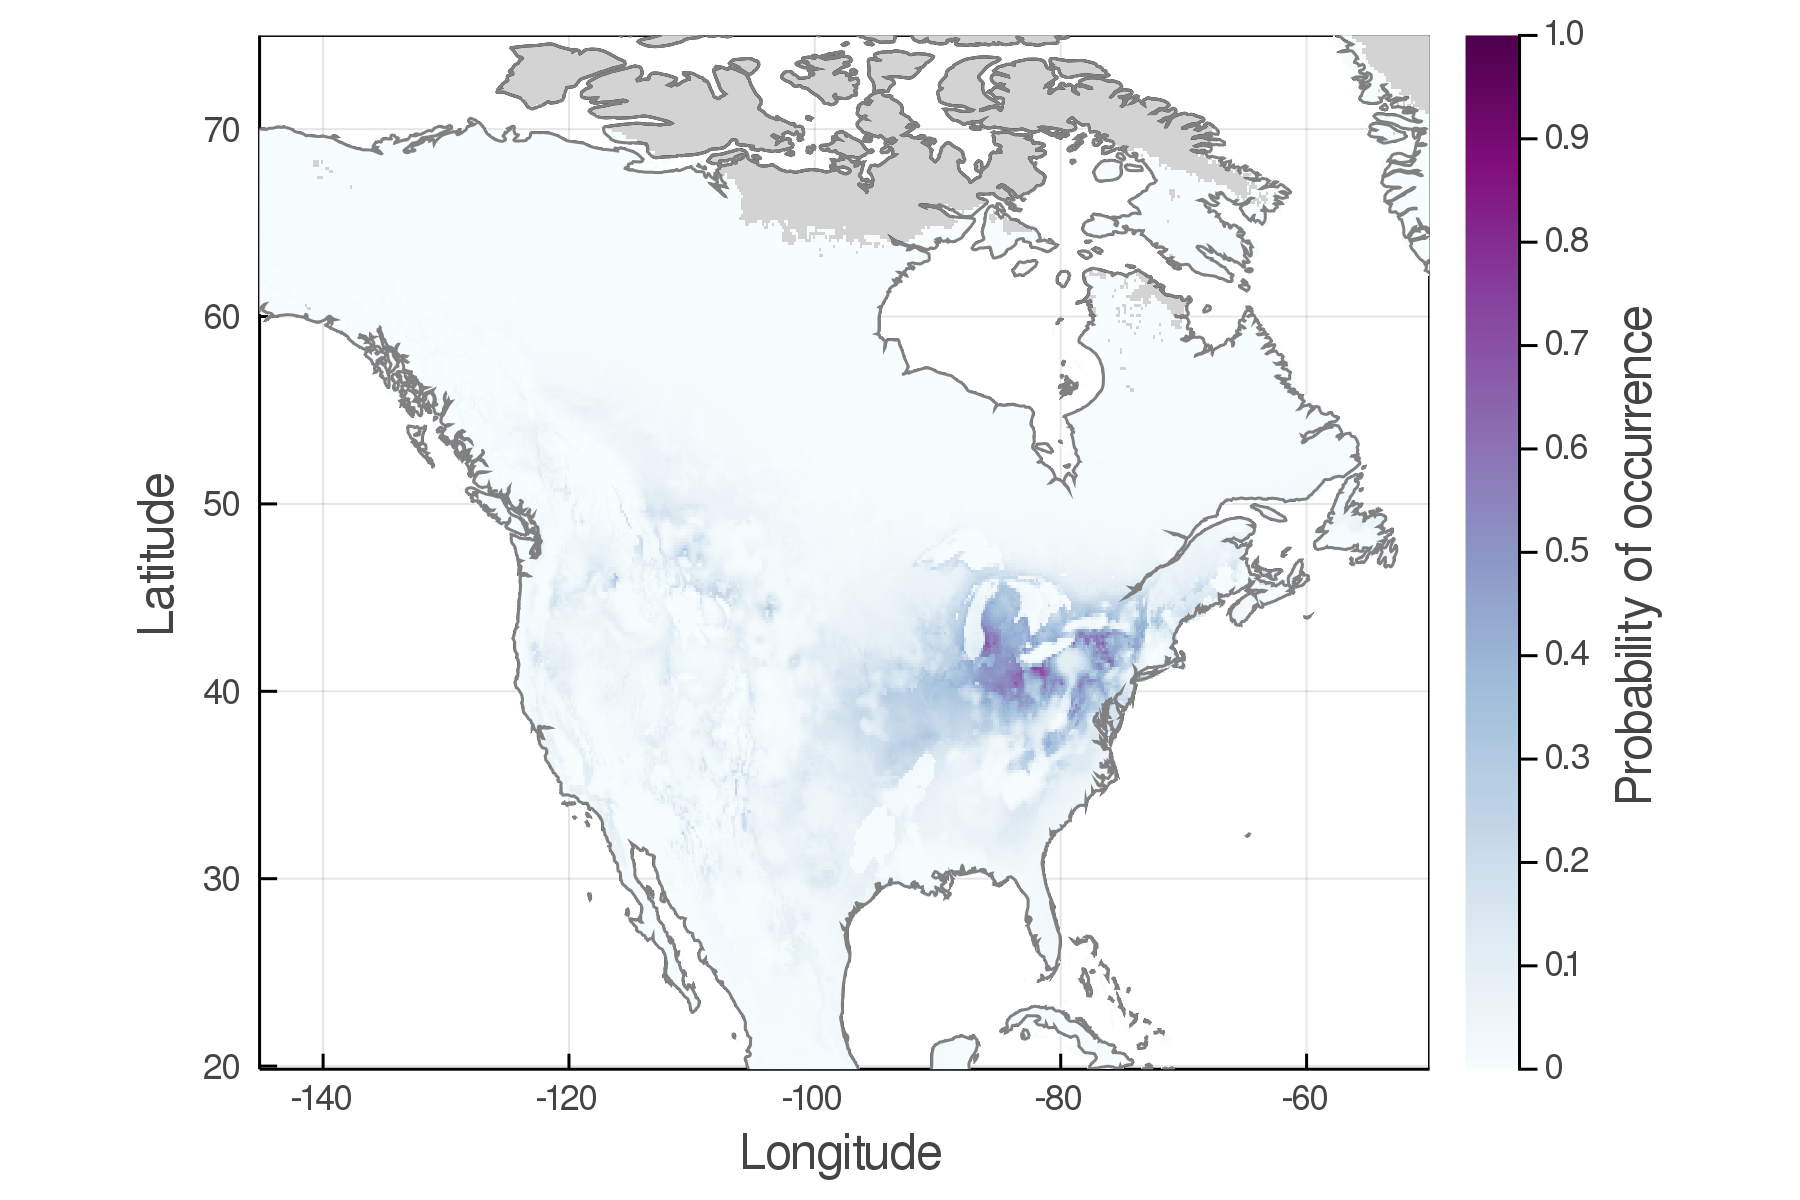
\includegraphics[scale=0.17]{fig/01_sdm_singlesp.png}
    \caption{SDM predictions without threshold for the Yellow Warbler}
  \end{figure}
\end{frame}

\begin{frame}
  \frametitle{Species richness - Raw data}
  \begin{figure}
    \centering
    \hspace*{-0cm}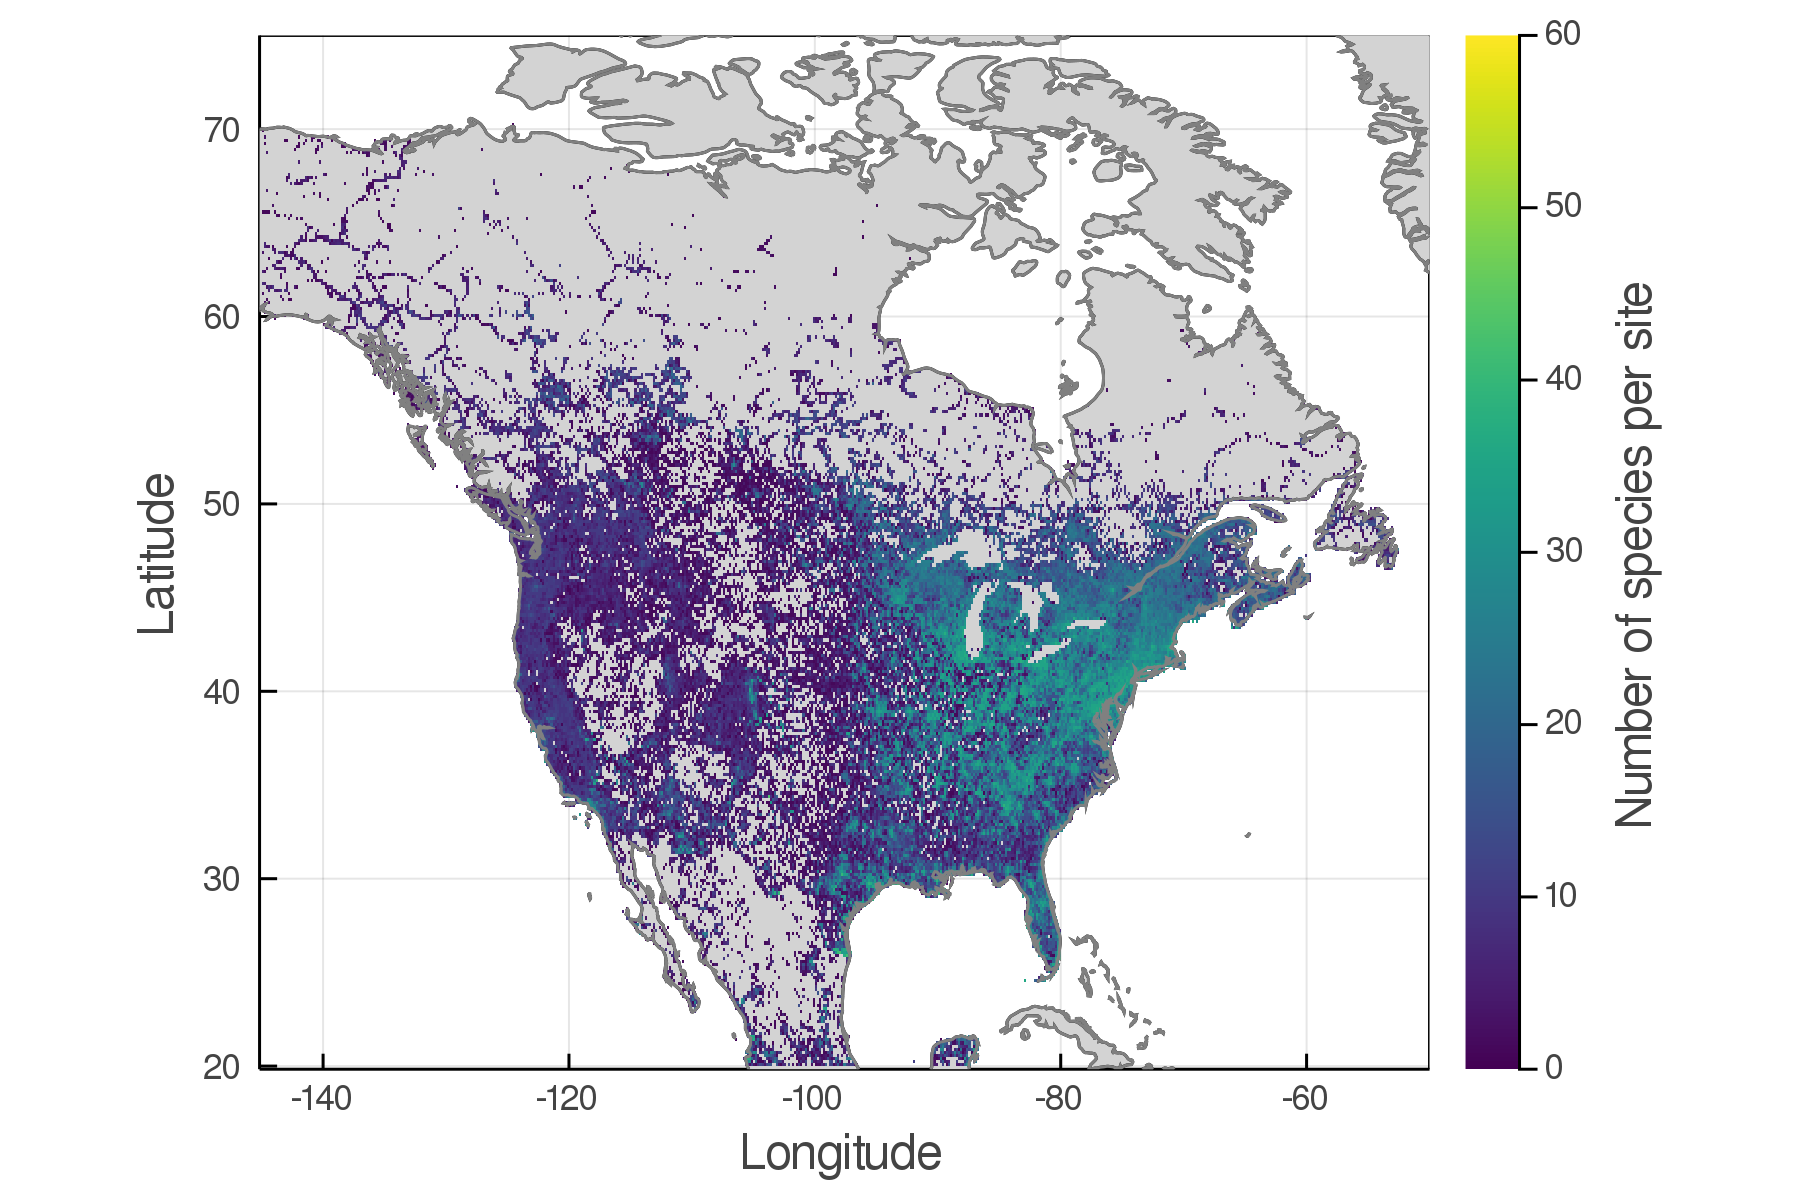
\includegraphics[scale=0.17]{fig/03_raw_richness.png}
  \end{figure}
\end{frame}

\begin{frame}
  \frametitle{Species richness - SDM}
  \begin{figure}
    \centering
    \hspace*{-0cm}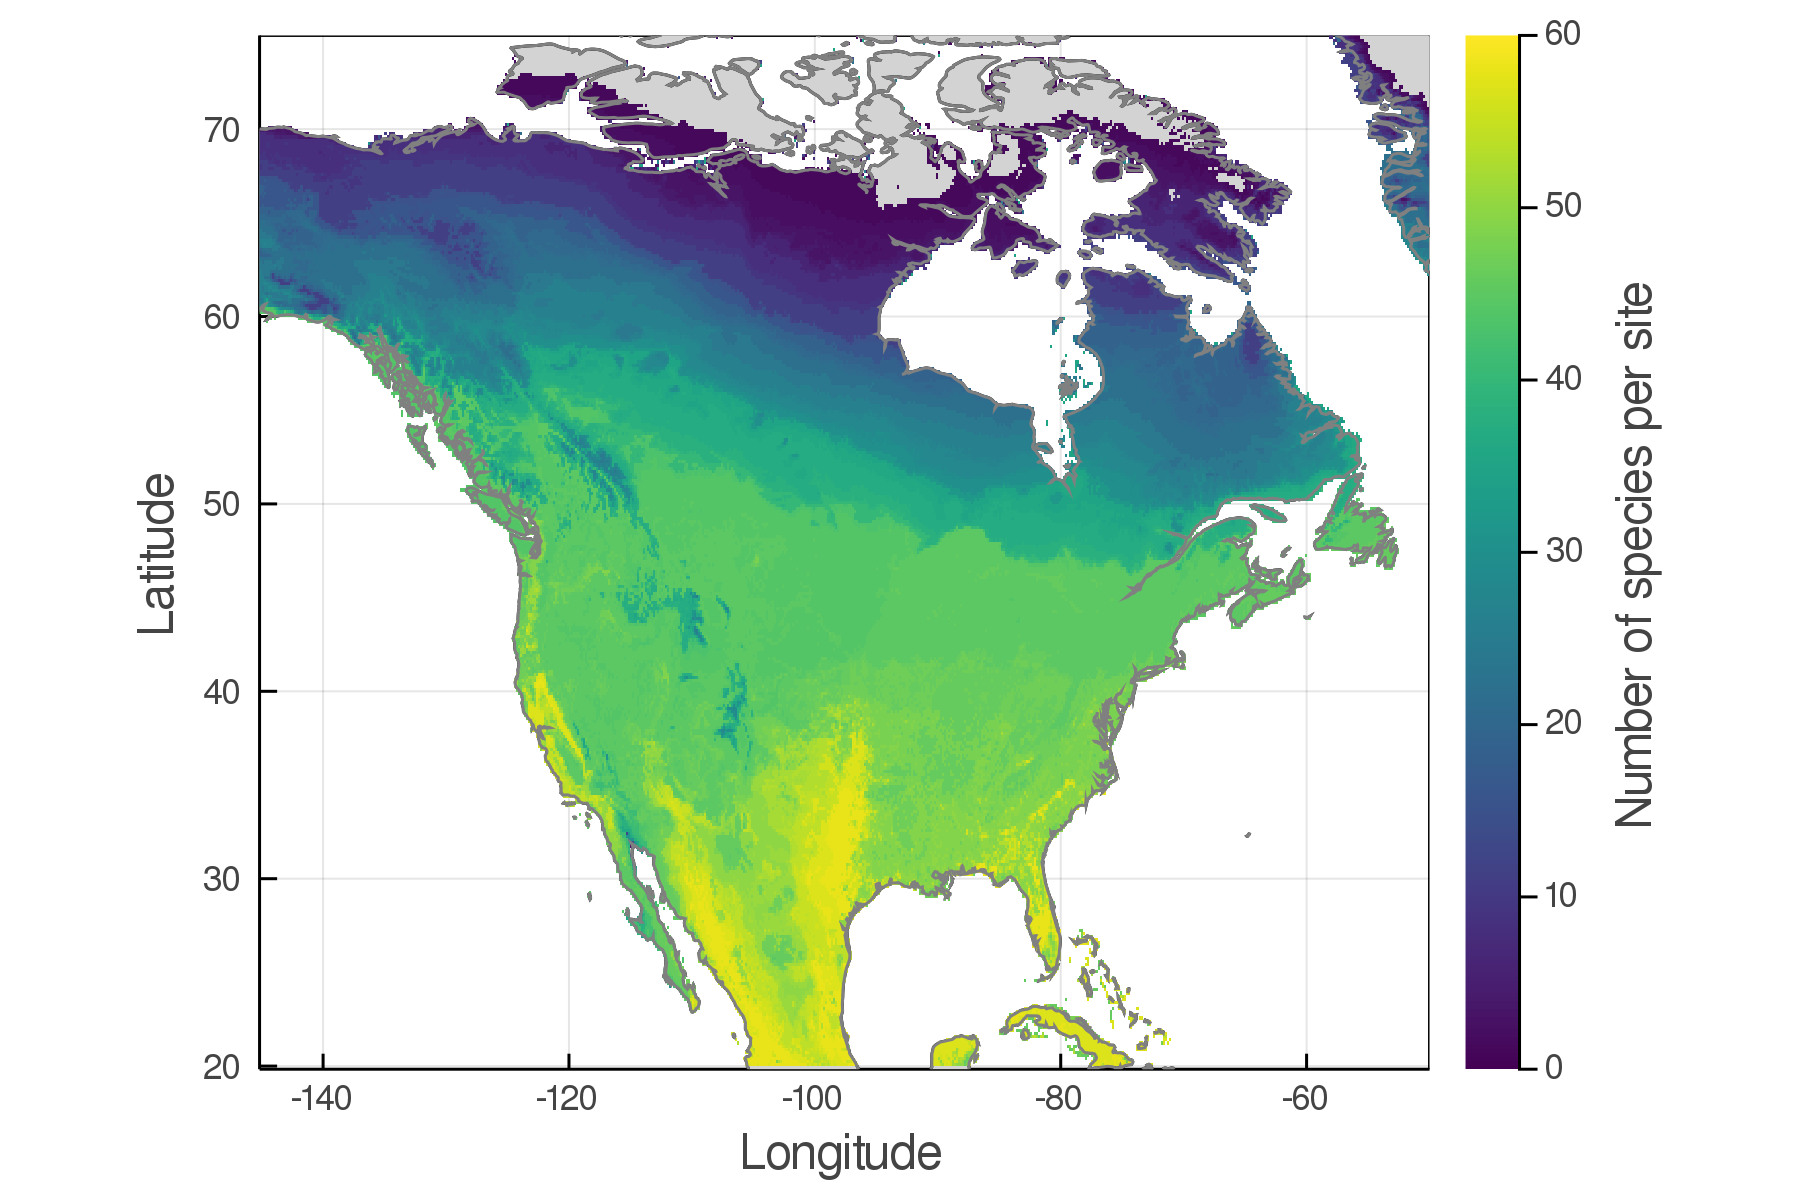
\includegraphics[scale=0.17]{fig/03_sdm_richness.png}
  \end{figure}
\end{frame}

\begin{frame}
  \frametitle{LCBD - Raw data (with Hellinger transformation)}
  \begin{figure}
    \centering
    \hspace*{-0cm}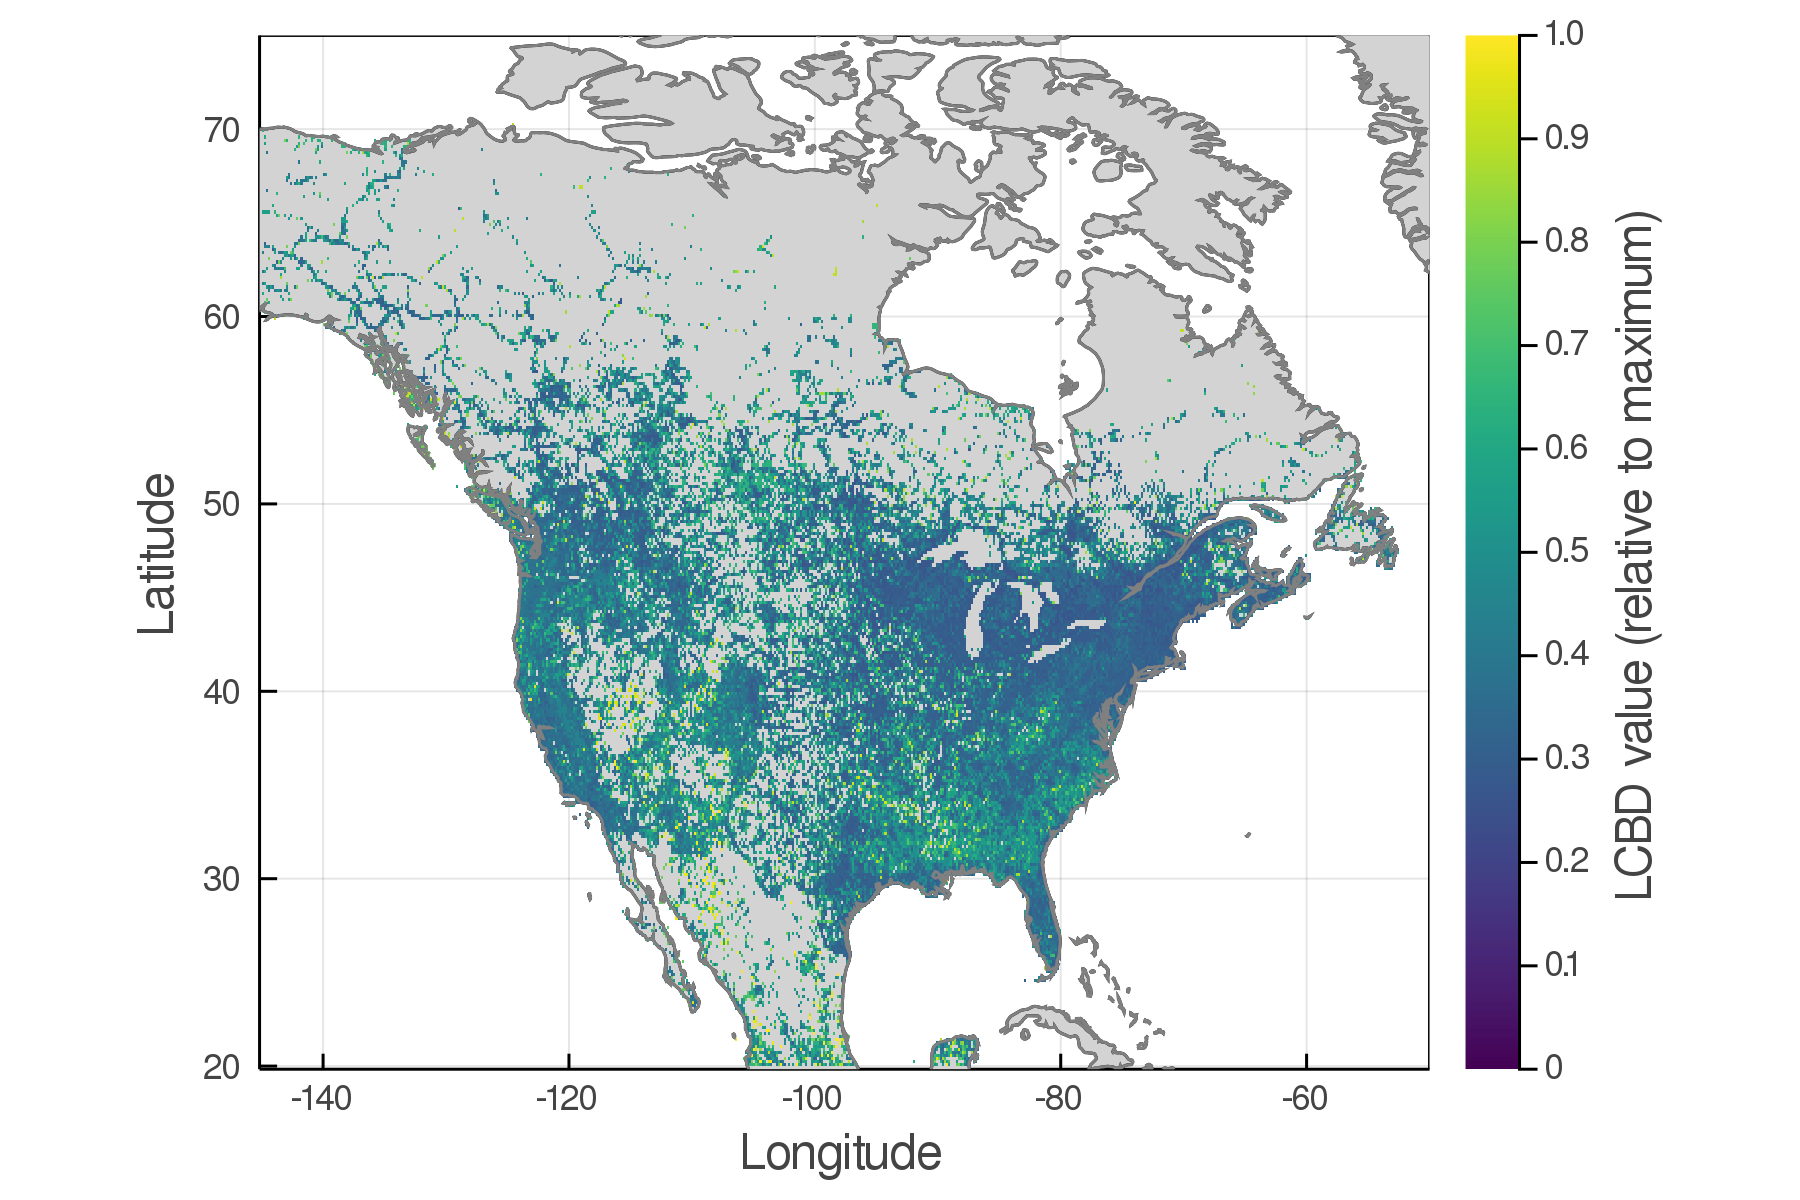
\includegraphics[scale=0.17]{fig/05_raw_lcbd-transf.png}
  \end{figure}
\end{frame}

\begin{frame}
  \frametitle{LCBD - SDM (no transformation)}
  \begin{figure}
    \centering
    \hspace*{-0cm}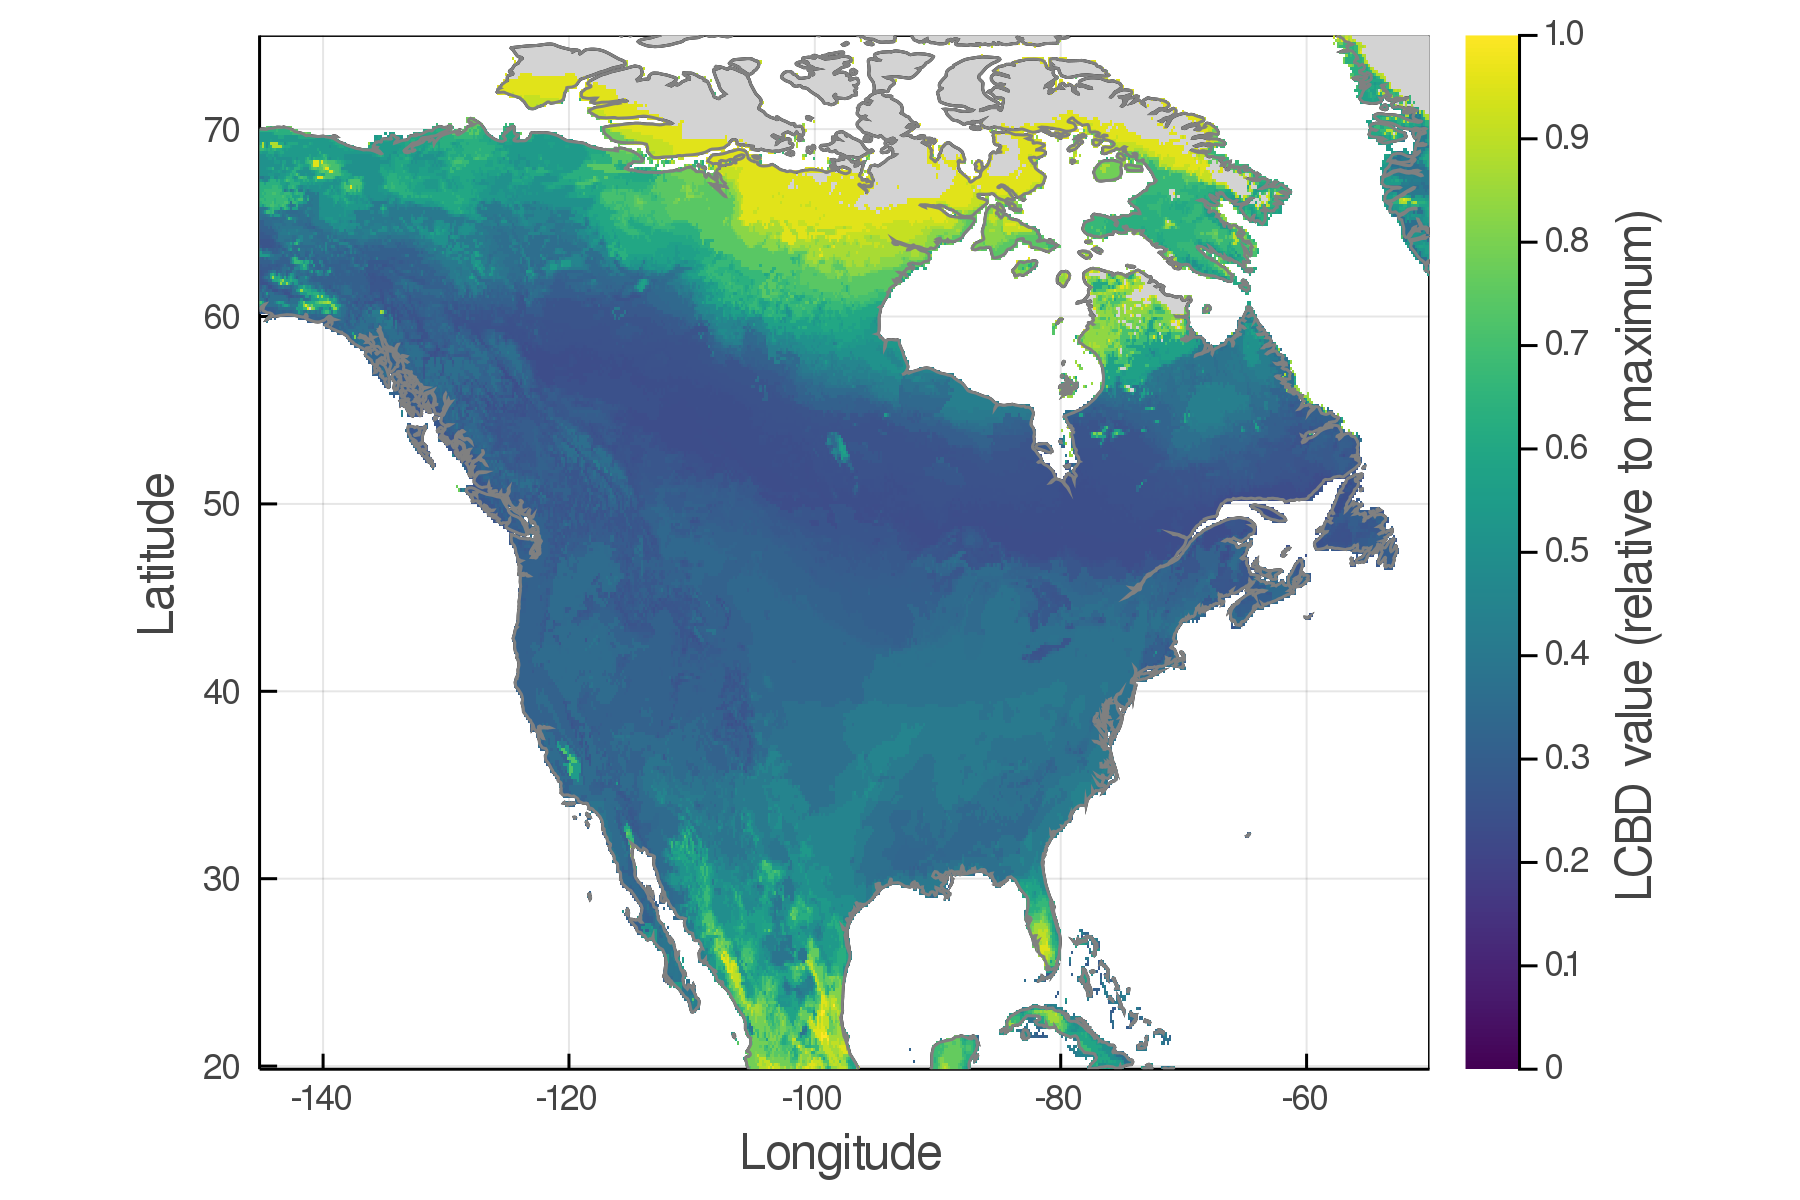
\includegraphics[scale=0.17]{fig/05_sdm_lcbd.png}
  \end{figure}
\end{frame}

\begin{frame}
  \frametitle{LCBD-richness relationship}
  \begin{figure}
    \centering
    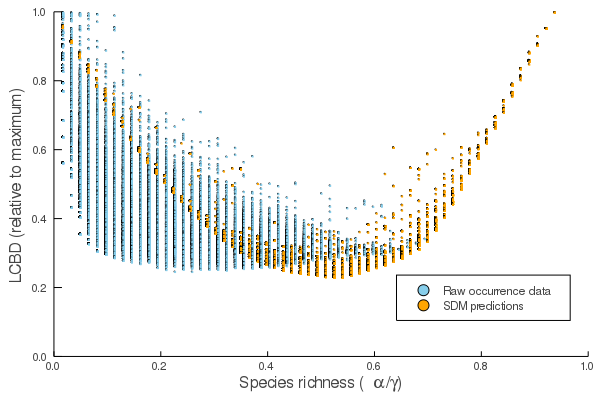
\includegraphics[scale=0.4]{fig/06_cmb_relation-oneplot.png}
  \end{figure}
\end{frame}

\end{document}
